%%=============================================================================
%% CAPITULO 2 -- REFERENCIAL TEORICO
%%
%% Esta e a parte do trabalho que mais demanda dominio das regras de citacao
%% (diretas e indiretas). Reveja a NBR 10520 antes de escrever.
%%=============================================================================

\section{Referencial teórico}

A transformação digital do setor público tem ampliado significativamente a disponibilidade de bases de dados governamentais capazes de subsidiar processos decisórios baseados em evidências. Nesse contexto, a Ciência de Dados, a Inteligência Artificial e as técnicas de Big Data assumem papel estratégico ao possibilitar a extração de conhecimento a partir de grandes volumes de dados estruturados e não estruturados. No setor da construção civil, essa realidade torna-se especialmente relevante diante da crescente complexidade dos investimentos públicos em infraestrutura e da necessidade de aprimorar mecanismos de planejamento, monitoramento e controle de custos. O Sistema Nacional de Pesquisa de Custos e Índices da Construção Civil (SINAPI), mantido pela Caixa Econômica Federal em parceria com o Instituto Brasileiro de Geografia e Estatística (IBGE), constitui a principal referência nacional para elaboração de orçamentos de obras públicas e apresenta características que o qualificam como uma importante fonte de dados para aplicações de Inteligência Artificial voltadas ao apoio à formulação e avaliação de políticas públicas.

\section{Políticas Públicas Baseadas em Evidências e Ciência de Dados}

A utilização de dados na formulação de políticas públicas ganhou relevância nas últimas décadas com o avanço da capacidade de armazenamento e processamento computacional. Segundo \citeonline{janssen2017bigdata}, a qualidade das decisões orientadas por dados depende da qualidade dos dados disponíveis, da governança informacional e da capacidade institucional de transformar informações em conhecimento aplicável à gestão pública.

Nesse contexto, o conceito de Big Data ultrapassa a simples acumulação de grandes volumes de informações e passa a envolver mecanismos capazes de gerar valor público por meio da análise de dados. A aplicação dessas técnicas permite identificar padrões, tendências e anomalias que dificilmente seriam percebidos por métodos convencionais de análise.

Para o setor público, a adoção dessas abordagens representa uma oportunidade de aprimorar a eficiência na aplicação dos recursos, reduzir riscos de execução e fortalecer mecanismos de transparência e controle. No caso específico desta pesquisa, tais benefícios podem ser observados na utilização dos dados do SINAPI para previsão de custos da construção civil e planejamento de investimentos governamentais.

\section{O SINAPI como Base Estratégica para Apoio à Decisão}

O Sistema Nacional de Pesquisa de Custos e Índices da Construção Civil (SINAPI) constitui a principal referência de preços e custos da construção civil utilizada pela administração pública brasileira. Segundo a \citeonline{caixaSINAPI}, o sistema reúne mensalmente informações sobre insumos, composições e índices de custos para todas as unidades da federação, servindo como base para orçamentos, medições e fiscalização de obras públicas.

A relevância estratégica do SINAPI foi reforçada pela própria Caixa Econômica Federal ao lançar, em 2026, iniciativa voltada à modernização do sistema por meio do Certame nº 0071/2026. A proposta reconhece a necessidade de ampliar as possibilidades de utilização dos dados e incentivar o desenvolvimento de soluções tecnológicas capazes de gerar inteligência para o setor da construção civil.

Apesar de sua ampla utilização institucional, o SINAPI permanece predominantemente voltado à consulta de informações históricas. Dessa forma, permanece pouco explorado o potencial da base para aplicações preditivas capazes de antecipar tendências, estimar custos futuros e subsidiar decisões relacionadas à alocação de recursos públicos.

A partir dessa perspectiva, esta pesquisa propõe a utilização dos dados do SINAPI como insumo para modelos estatísticos espaço-temporais e algoritmos de inteligência artificial, buscando transformar uma base tradicionalmente consultiva em um instrumento de apoio à tomada de decisão em políticas públicas de infraestrutura. A Figura \ref{fig:arquitetura_sinapi} apresenta a arquitetura conceitual que orienta o desenvolvimento desta pesquisa.

%% --- Exemplo de figura com legenda ACIMA e fonte ABAIXO --------------------
\begin{figure}[htb]
  \caption{Arquitetura conceitual da aplicação de inteligência artificial aos dados do SINAPI para apoio à tomada de decisão em políticas públicas}
  \label{fig:arquitetura_sinapi}
  \centering
  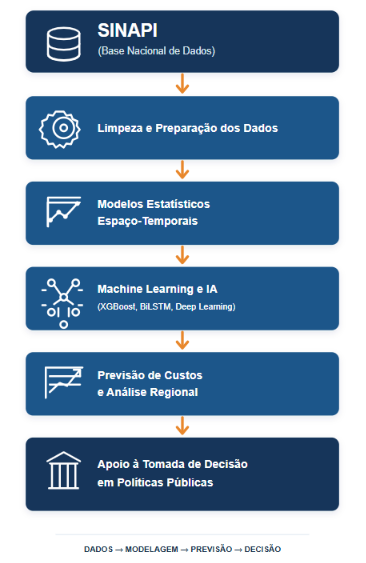
\includegraphics[width=0.8\textwidth]{figuras/infografico-fluxo-sinapi.png}
  \fonte{Elaborado pela autora com auxílio do Copilot (2026).}
\end{figure}


\section{Inteligência Artificial e Machine Learning na Previsão de Custos}

A evolução dos modelos computacionais impulsionou a utilização de técnicas de Inteligência Artificial para problemas de previsão em diferentes áreas do conhecimento. Conforme destacam \citeonline{goodfellow2016deeplearning}, algoritmos de Deep Learning apresentam elevada capacidade de identificar padrões complexos e relações não lineares em grandes conjuntos de dados.

No campo da construção civil, a literatura recente demonstra crescente utilização de técnicas de Machine Learning para estimativa e previsão de custos. \citeonline{karadimos2024taxonomy} identificam uma ampla variedade de algoritmos aplicados ao problema, incluindo redes neurais artificiais, árvores de decisão, métodos de ensemble learning e modelos híbridos.

Resultados semelhantes são apresentados por \citeonline{shamim2025advancement}, que demonstram o crescimento da utilização de técnicas de Machine Learning e Deep Learning em projetos de engenharia, destacando ganhos de precisão quando comparados aos métodos tradicionais de estimação de custos.

Tais evidências reforçam a hipótese desta pesquisa de que modelos avançados de Inteligência Artificial podem aumentar a capacidade preditiva do SINAPI e contribuir para o aprimoramento do planejamento orçamentário e da gestão de riscos em projetos de infraestrutura.

\subsection{Modelos Temporais Aplicados à Construção Civil}

A análise temporal dos custos representa um dos principais desafios para a gestão de obras e investimentos públicos. Nesse contexto, \citeonline{wang2024bilstm} demonstram que modelos baseados em redes neurais Bidirectional Long Short-Term Memory (BiLSTM) apresentam elevada capacidade para capturar padrões temporais complexos na evolução dos custos da construção civil.

Os resultados obtidos pelos autores indicam que arquiteturas de aprendizado profundo podem identificar tendências e ciclos econômicos que influenciam o comportamento dos preços, ampliando a precisão dos modelos de previsão em comparação a abordagens tradicionais.

\subsection{Modelos Espaço-Temporais e Diferenças Regionais}

A literatura recente reconhece que a dimensão geográfica exerce influência significativa sobre o comportamento dos custos da construção civil. Fatores como disponibilidade de insumos, características logísticas, condições econômicas locais e aspectos regionais afetam diretamente a formação dos preços.

Nesse sentido, \citeonline{mostofi2026bilstm} desenvolveram modelos espaço-temporais baseados em Deep Learning capazes de incorporar simultaneamente características geográficas e temporais para previsão de desempenho de custos em projetos de construção. Os resultados evidenciam ganhos relevantes de precisão quando comparados a modelos que consideram apenas a dimensão temporal.

Essa abordagem apresenta especial relevância para esta pesquisa, considerando que um dos objetivos consiste em investigar se a utilização de valores de referência da região de São Paulo para localidades sem observações próprias pode introduzir distorções nos orçamentos públicos e impactar a eficiência da alocação de recursos governamentais.

\section{Aplicações de Inteligência Artificial em Projetos de Infraestrutura}

De forma complementar, \citeonline{antoniou2025highway} desenvolveram modelos de aprendizado de máquina voltados à previsão de custos de rodovias, demonstrando que algoritmos baseados em aprendizado supervisionado podem fornecer estimativas confiáveis já nas fases iniciais de planejamento.

Esses estudos reforçam o potencial da aplicação de técnicas avançadas de análise de dados em bases públicas de custos, indicando oportunidades para ampliar o uso do SINAPI como ferramenta de inteligência para apoio à tomada de decisão em políticas públicas de infraestrutura.

\section{Síntese da Literatura e Lacuna de Pesquisa}

A revisão da literatura evidencia que a utilização de Inteligência Artificial, Machine Learning e modelos espaço-temporais para previsão de custos em projetos de engenharia constitui uma área de pesquisa em rápida expansão. Os trabalhos analisados demonstram ganhos consistentes na precisão das estimativas e na capacidade de antecipação de riscos.

Contudo, observa-se que a maior parte das pesquisas foi desenvolvida utilizando bases proprietárias ou conjuntos de dados internacionais. Permanecem escassos os estudos que exploram bases públicas nacionais de ampla abrangência territorial para suporte à formulação de políticas públicas.

Diante desse cenário, esta pesquisa busca preencher essa lacuna por meio da aplicação de modelos estatísticos espaço-temporais, Machine Learning e Big Data sobre os dados do SINAPI, avaliando tanto sua capacidade de produzir previsões confiáveis de custos quanto seu potencial para identificar distorções regionais de preços que possam impactar a eficiência das contratações públicas e a formulação de políticas públicas de infraestrutura.





%% --- Exemplo de quadro -----------------------------------------------------
\begin{quadro}[htb]
  \caption{Título do quadro}
  \label{qua:exemplo}
  \centering
  \begin{tabular}{ll}
    \toprule
    \textbf{Elemento} & \textbf{Norma aplicável} \\
    \midrule
    Trabalhos acadêmicos & NBR 14724 \\
    Referências          & NBR 6023  \\
    Citações             & NBR 10520 \\
    Sumário              & NBR 6027  \\
    Resumo               & NBR 6028  \\
    \bottomrule
  \end{tabular}
  \fonte{Elaborado pelo autor (\the\year).}
\end{quadro}

%% --- Exemplo de tabela -----------------------------------------------------
\begin{table}[htb]
  \caption{Nome da Tabela 1}
  \label{tab:exemplo}
  \centering
  \begin{tabular}{lrr}
    \toprule
    \textbf{Categoria} & \textbf{Frequência} & \textbf{\%} \\
    \midrule
    Categoria A & 120 & 40,0 \\
    Categoria B &  90 & 30,0 \\
    Categoria C &  90 & 30,0 \\
    \midrule
    \textbf{Total} & \textbf{300} & \textbf{100,0} \\
    \bottomrule
  \end{tabular}
  \fonte{Dados da pesquisa (\the\year).}
\end{table}

%% --- Exemplo de grafico ----------------------------------------------------
\begin{grafico}[htb]
  \caption{Nome do Gráfico 1}
  \label{gra:exemplo}
  \centering
  \includegraphics[width=0.55\textwidth]{figuras/exemplo-figura.png}
  \fonte{Elaborado pelo autor (\the\year).}
\end{grafico}
